\documentclass[10pt,a4paper]{article}
\usepackage[a4paper, top=2cm, bottom=1.5cm, left=1.5cm, right=1.5cm]{geometry} % Задать размеры полей.
\usepackage[warn]{mathtext} % Русские символы в формулах. Нужно писать до пакета babel. Указывает, что в формулах используются символы кириллицы, которые по умолчанию печатаются прямым шрифтом.
\usepackage[T2A]{fontenc}
\usepackage[utf8]{inputenc}
\usepackage[russian]{babel}
\usepackage{amsmath}
\usepackage{amssymb}
\usepackage{graphicx}
\usepackage{floatrow}
\usepackage{booktabs}
\usepackage{wrapfig}
\usepackage{lipsum}
%\usepackage{subcaption}
\usepackage{fancyhdr}
\usepackage{multicol}
\usepackage{xcolor}

%multi-column
%\multicolumn{number cols}{align}{text} % align: l,c,r

%multi-row
\usepackage{multirow}

\newcommand{\figref}[1]{(См. рис. \ref{#1})}
\newcommand{\secref}[1]{(См. раздел. \ref{#1})}

\newcommand{\e}[1]{\text{$\cdot10^{#1}$}}
\newcommand{\m}{\; м}
\newcommand{\mm}{\; мм}
\newcommand{\um}{\; мкм}
\newcommand{\A}{\; А}
\newcommand{\uV}{\; мкВ}
\newcommand{\cels}{\; ^\circ С}

\newcommand{\assert}[1] {
	\Huge 
	\color{red}
	\text{#1}
	\color{black}
	\normalsize	
}

\pagestyle{fancy}
\fancyhead{}
\fancyhead[L]{\small Маслов А.С., Дедков Д.А., Экспериментальная проверка закона Стефана-Больцмана, и определение постоянных Стефана-Больцмана и Планка из анализа теплового излучения раскалённой вольфрамовой нити. МФТИ, 2023 г.}
\fancyhead[R]{}
\fancyfoot[C]{\thepage}

\renewcommand{\cot}{\text{ctg}}

\author{\normalsize Маслов Артём, Дедков Денис \\
	\normalsize группа Б01-108а \\
	\normalsize 04.09.2023}
\date{}

\usepackage{float}
\restylefloat{table}
\title{
	\Large \assert{Артем, для тебя} \\ 
} 

\addto\captionsrussian{\def\refname{Литература}}

\begin{document}
\maketitle
\begin{multicols}{2}
	
	\subsection*{Аннотация}
	\assert{Артем, для тебя :)}
	
	\subsection*{Введение}
	\assert{Артем, для тебя :)}
	
	\subsection*{Описание экспериментальной установки}
	\assert{Артем, для тебя :)}
		
	\subsection*{Оборудование и приборы}
	\assert{Артем, для тебя :)}
	
	\subsection*{Методика эксперимента}
	\assert{Артем, для тебя :)}
	
	\subsection*{Экспериментальные результаты}
		
	\subsubsection*{Калибровка детектора}
	Зная значения энергии $\alpha$-частицы при распаде $\text{Ra}_{88}^{226}$ и его дочерних ядер, можно определить коэффициенты в зависимости энергии $E_i$ от номера канала спектрометра $N_i$:
	
	$$E_i = a\cdot N_i + b.$$
	
	График $E_i(N_i)$ изображен на рисунке \ref{fig:w-channel}. Методом наименьших квадратов были получены следующие численные значения:
	
	$$ a = (2.97 \pm 0.01) \cdot 10^{-3} \; \frac{ \text{МэВ} }{ \text{кан.} },$$
	$$ b = (-0.10 \pm 0.02) \; \text{МэВ}.$$
	
	\begin{figure}[H]
		\includegraphics[width=1\textwidth]{gen/fig-w-channel.pdf}
		\caption{Зависимость энергии $\alpha$-частицы от номера канала $E_i(N_i)$.}
		\label{fig:w-channel}
	\end{figure}

	Следует обратить внимание на систематический сдвиг $b$ по энергии, которого в теории быть не должно. В данном случае проблематично понять, является ли этот сдвиг постоянным для данного прибора, или это систематика, появляющаяся при ручных изменениях в установке. Систематическая ошибка, вносимая этим сдвигом $\varepsilon \sim 2\%$. В таблицах будет вычислена случайная составляющая ошибок, чтобы иметь представление об их порядке. Полная погрешность оценивается по формуле:
	
	$$\varepsilon_\Sigma = \sqrt{\varepsilon^2 + \varepsilon_{E_i}^2}$$
	
	\subsubsection*{Изучение спектров $\alpha$-распада}
			
	Используя калибровочный график, можно определить значения энергии для всех остальных элементов: $\text{Ra}_{88}^{226}$, $\text{Am}_{95}^{241} + \text{Th}_{90}^{230}$, $\text{Pu}_{94}^{239}$, $\text{U}_{\text{пр}}$.
	
	В соответствующих таблицах приведены номер канала $N_i$, ширина пика $\Delta N_i$, энергия $E_i$, ширина $\Delta E_i$. А также случайная составляющая относительной ошибки пересчета номера канала в энергию.
	
	Энергетическое разрешение вычисляется по следующей формуле:
	$$R_i = \frac{\Delta E_i}{E_i}$$
	
	Оценку влияния статистической флуктуации числа электрон-дырочных пар, создаваемых падающей частицей можно получить с помощью следующей формулы:
	
	$$R_{f,i} = \sqrt{\frac{E_{\text{ср}}}{E_i}} \approx \sqrt{\frac{3.6\; \text{эВ}}{E_i}}$$

	Оценку погрешности проводим с помощью оценки косвенных измерений:
	
	$$ \varepsilon_{R_{f,i}} = \frac{1}{2} \sqrt{\varepsilon_\Sigma^2 + \left(\frac{0.05}{3.60}\right)^2} \sim 1.5 \%$$

		
	$$ \varepsilon_{R_i} = \sqrt{\varepsilon_{E_i}^2 + \varepsilon_{\Sigma}^2} \approx  \varepsilon_{\Sigma} \sim 2 \%$$

	Значения энергетического разрешения также приведены в таблицах.

	\subsubsection*{Изучение $\alpha$-распада $\text{Ra}_{88}^{226}$}
	
	\begin{figure}[H]
		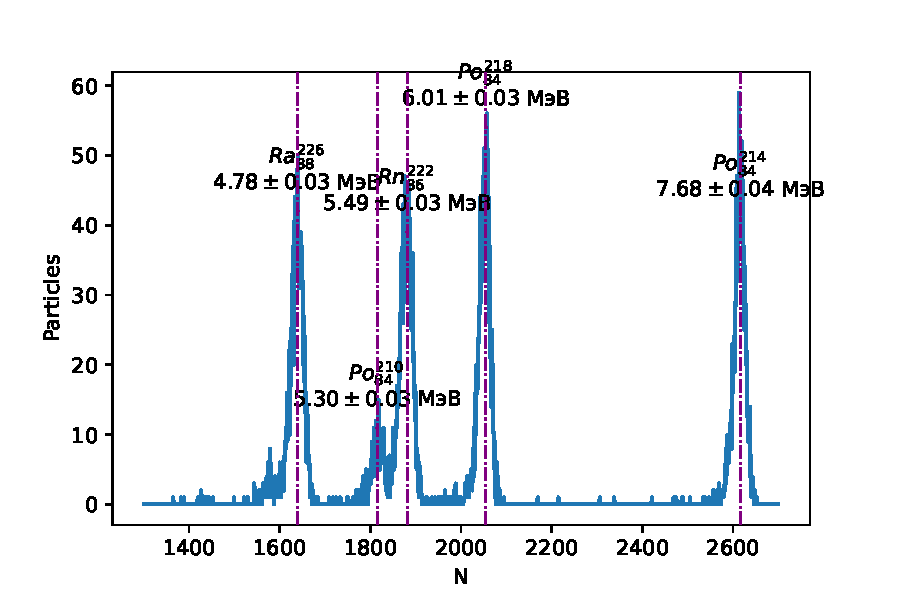
\includegraphics[width=1\textwidth]{gen/fig-ra.pdf}
		\caption{Спектр $\text{Ra}_{88}^{226}$.}
		\label{fig:ra}
	\end{figure}
	
	\begin{table}[H]
		\addtolength{\tabcolsep}{-4pt}
		\footnotesize
		\begin{tabular}{cccccc}
\toprule
$N_i$ & $dN_i$ & $E_i$, МэВ & $\sigma_{E_i}$, МэВ & $\Delta E_i$, МэВ & $\sigma_{\Delta E_i}$, МэВ \\
\midrule
1640.0 & 24.33 & 4.78 & 0.03 & 0.0723 & 0.0003 \\
1815.0 & 22.58 & 5.30 & 0.03 & 0.0671 & 0.0002 \\
1881.0 & 23.97 & 5.49 & 0.03 & 0.0712 & 0.0003 \\
2055.0 & 21.05 & 6.01 & 0.03 & 0.0626 & 0.0002 \\
2617.0 & 22.50 & 7.68 & 0.04 & 0.0669 & 0.0002 \\
\bottomrule
\end{tabular}

		\caption{Энергии пиков $\text{Ra}_{88}^{226}$.}
		\label{tab:term}
	\end{table}


	\subsubsection*{Изучение $\alpha$-распада $\text{Am}_{95}^{241} + \text{Th}_{90}^{230}$}

	\begin{figure}[H]
		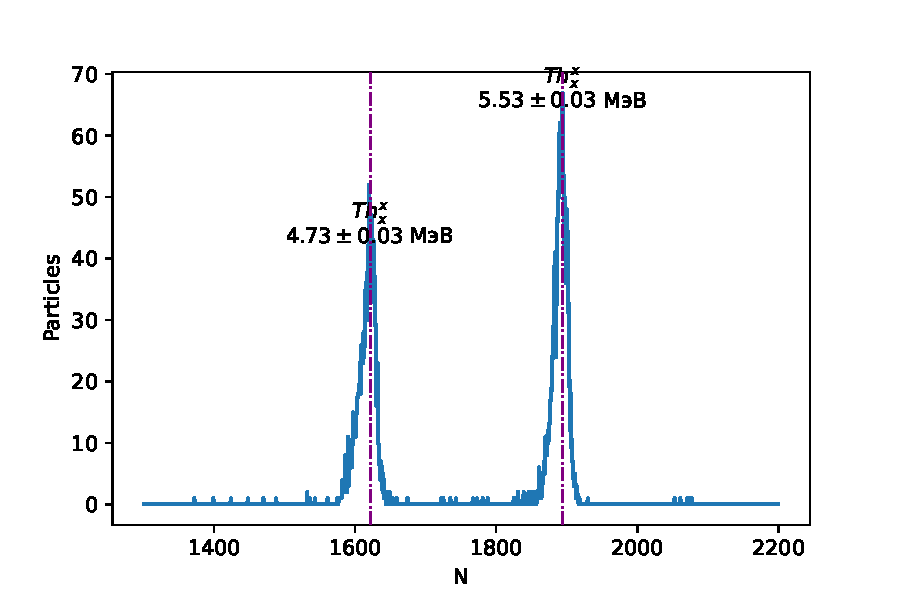
\includegraphics[width=1\textwidth]{gen/fig-th_am.pdf}
		\caption{Спектр $\text{Am}_{95}^{241} + \text{Th}_{90}^{230}$.}
		\label{fig:th_am}
	\end{figure}
	
	\begin{table}[H]
		\addtolength{\tabcolsep}{-4pt}
		\footnotesize
		\begin{tabular}{ccccccc}
\toprule
$N_i$ & $\Delta N_i$ & $E_i$, МэВ & $\varepsilon_{E_i}, \%$ & $\Delta E_i$, МэВ & $R_i \cdot 10^2$ & $R_{f,i} \cdot 10^2$ \\
\midrule
1622 & 15.80 & 4.73 & 0.6 & 0.0469 & 0.99 & 0.087 \\
1894 & 17.12 & 5.53 & 0.6 & 0.0509 & 0.92 & 0.081 \\
\bottomrule
\end{tabular}

		\caption{Энергии пиков $\text{Am}_{95}^{241} + \text{Th}_{90}^{230}$.}
		\label{tab:th_am}
	\end{table}
	
	
	\subsubsection*{Изучение $\alpha$-распада $\text{Pu}_{94}^{239}$}
	
	\begin{figure}[H]
		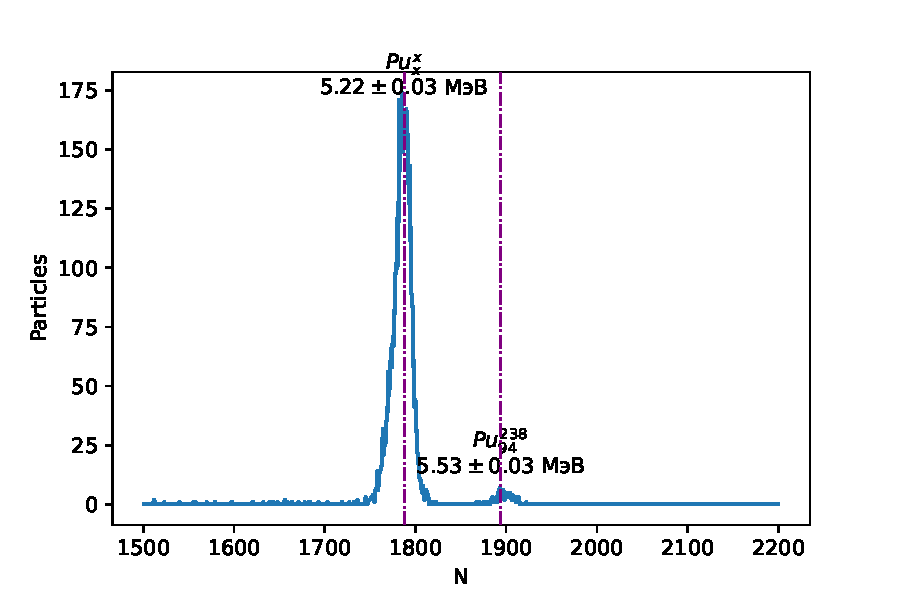
\includegraphics[width=1\textwidth]{gen/fig-pu.pdf}
		\caption{Спектр $\text{Pu}_{94}^{239}$.}
		\label{fig:pu}
	\end{figure}
	
	\begin{table}[H]
		\addtolength{\tabcolsep}{-4pt}
		\footnotesize
		\begin{tabular}{ccccccc}
\toprule
$N_i$ & $\Delta N_i$ & $E_i$, МэВ & $\varepsilon_{E_i}, \%$ & $\Delta E_i$, МэВ & $R_i \cdot 10^2$ & $R_{f,i} \cdot 10^2$ \\
\midrule
1788 & 16.81 & 5.22 & 0.6 & 0.0500 & 0.96 & 0.083 \\
1894 & 20.90 & 5.53 & 0.6 & 0.0621 & 1.12 & 0.081 \\
\bottomrule
\end{tabular}

		\caption{Энергии пиков $\text{Pu}_{94}^{239}$.}
		\label{tab:pu}
	\end{table}
	
	
	\subsubsection*{Изучение $\alpha$-распада $\text{U}_{\text{пр}}$}
	
	\begin{figure}[H]
		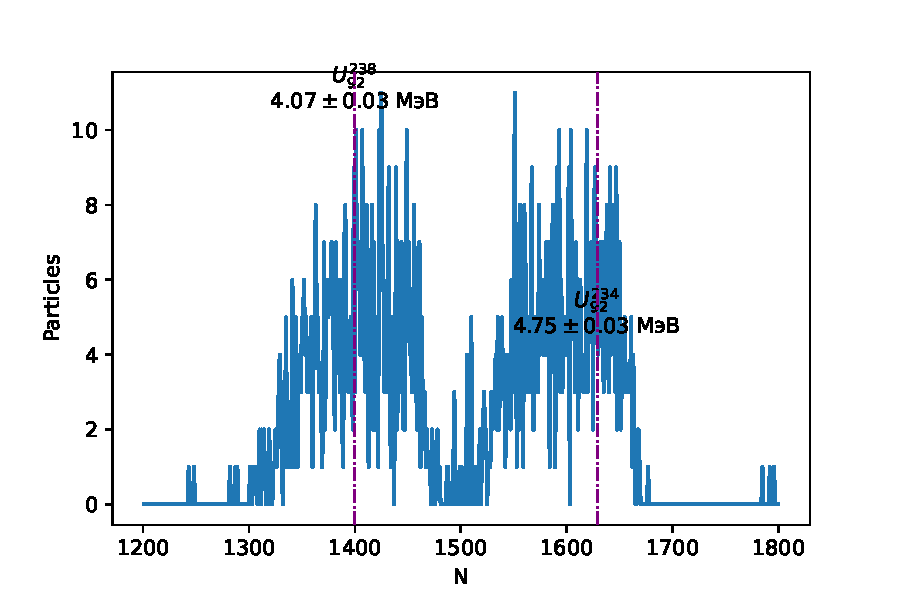
\includegraphics[width=1\textwidth]{gen/fig-u.pdf}
		\caption{Спектр $\text{U}_{\text{пр}}$.}
		\label{fig:u}
	\end{figure}
	
	\begin{table}[H]
		\addtolength{\tabcolsep}{-4pt}
		\footnotesize
		\begin{tabular}{ccccccc}
\toprule
$N_i$ & $\Delta N_i$ & $E_i$, МэВ & $\varepsilon_{E_i}, \%$ & $\Delta E_i$, МэВ & $R_i \cdot 10^2$ & $R_{f,i} \cdot 10^2$ \\
\midrule
1400 & 87.96 & 4.07 & 0.7 & 0.2614 & 6.43 & 0.094 \\
1629 & 43.20 & 4.75 & 0.6 & 0.1284 & 2.71 & 0.087 \\
\bottomrule
\end{tabular}

		\caption{Энергии пиков $\text{U}_{\text{пр}}$.}
		\label{tab:u}
	\end{table}

	\subsubsection*{Проверка закона Гейгера-Нэттола}

	Зная энергии $\alpha$-распада $\text{Ra}_{88}^{226}$ и его дочерних ядер, а также периоды их полураспада, можно судить о точности выполнения закона Гейгера-Неттола. С этой целью проведем линеаризацию зависимости:
	
	$$\log{T_{1/2}} = \frac{a}{\sqrt{E_i}} + b.$$
	
	\begin{figure}[H]
		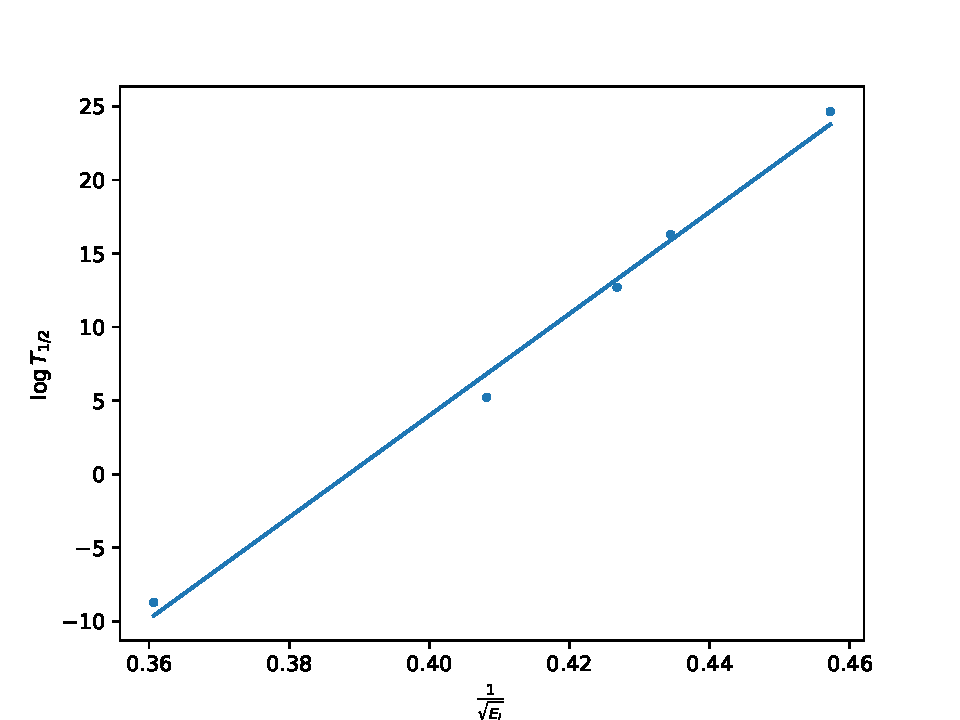
\includegraphics[width=1\textwidth]{gen/fig-te.pdf}
		\caption{График $\log{T_{1/2}} \left( \frac{1}{\sqrt{E_i}}\right)$.}
		\label{fig:te}
	\end{figure}
	
	Полученный график изображен на рисунке \ref{fig:te}. Коэффициент корреляции слабо отличается от единицы: 
	
	$$ \rho = \frac{ \text{cov}_{ xy } }{ \sigma_x \cdot \sigma_y} = 0.9964. $$
	
	\subsection*{Выводы}
	
	В работе предоставлены спектры $\alpha$-излучения ядер. Мы экспериментально определили энергетическое разрешение детектора (см. таблицы):
	
	$$R_i = \frac{\Delta E_i}{E_i},\; \varepsilon_{R_i} \sim 2 \%$$

	Оценка влияния статистической флуктуации числа электрон-дырочных пар $R_{f,i} = \sqrt{\frac{E_{\text{ср}}}{E_i}}, \; \varepsilon_{R_{f,i}} \sim 1.5 \%$, создаваемых падающей частицей, получилась на порядки меньше вычисленных энергетических разрешений $R_i$. Откуда можно сделать вывод, что основной причиной разброса импульсов по амплитуде является шум электрических цепей.
	
	
	Также проверен закон Гейгера-Нэттола методом линеаризации зависимости. Коэффициент корреляции слабо отличается от единицы: 
	
	$$ \rho (x,y) = 0.9964. $$
	
	
	
	\begin{thebibliography}{}
		\bibitem{labnik} \textbf{Ципенюк, Ю.М.} Лабораторный практикум по общей физике. Квантовая физика: Учеб. пособие для вузов./ Игошин~Ф.Ф., Самарский~Ю.А., Ципенюк~Ю.М.; Под. ред. Ципенюка~Ю.М. --- М.: Физматкнига, 2012. --- 464 с. ISBN 978-5-89155-206-7.
		\bibitem{Sivukhin4} \textbf{Сивухин, Д.В.} Общий курс физики: Учеб. пособие: Для вузов. В 5 т. Т.IV. Оптика. --- 4-е изд., стереот. --- М.: ФИЗМАТЛИТ, 2021. --- 792 с. ISBN 978-5-9221-1735-7 (Т. IV).
	\end{thebibliography}
\end{multicols}
\end{document}